\begin{savequote}
Apparently the child recognizes speech sounds as patterns of gestures.
\qauthor{Israel Rosenfield, \textit{The invention of memory}}
\end{savequote}
\chapter{Gesture modeling and recognition}

Compare temporal data modeling: HMM and CRF. 

\section{Temporal Gesture Modeling and Training}

Previous research suggests that
a gesture consists of three phases: \textit{pre-stroke}, \textit{nucleus}, and \textit{post-stroke}~\cite{Pavlovic97}. The pre-stroke phase consists
of a preparatory movement that sets the hand in motion from some resting position.
The nucleus of a gesture has some ``definite form and enhanced dynamic qualities''
~\cite{kendon86}. Finally, the hand either returns to the resting position or repositions
for the new gesture phase. Each gesture
phase includes a sequence of hand/arm movement that can be modeled using HMMs (see Figure~\ref{fig:hmm}). 
This means we can use model temporal gestures as hierarchical hidden Markov
models.

\begin{figure}[tbh]
\centering
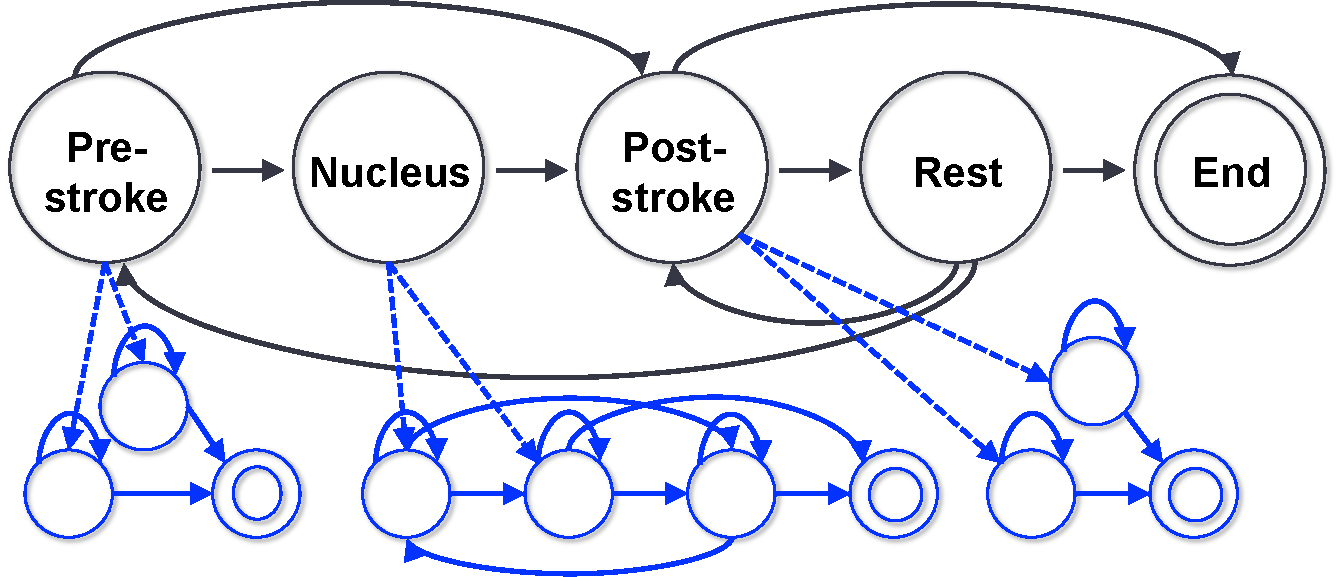
\includegraphics[clip, width=1\columnwidth]{figures/hmm.pdf}
\caption{Temporal gesture model with different phases. Each phase can be modeled as an HMM. Dashed arrows represent
initial state transitions and double circles
represent end states.}
\label{fig:hmm}
\end{figure}

The pre-stroke and post-stroke phases are basically transition phases. We
can also use them to model transitions between different rest positions. We
allow pre-stroke to terminate or go to post-stroke phase. We allow rest state to
go to pre- and post-stroke phases.

Because we have the ground truth labeling of pre-stroke, nucleus and post-stroke phases, 
we can train an HMM for each phase for each gesture. 

\section{Hierarchical Hidden Markov Models}
We combine different levels of recognition using the abstract hidden Markov
model (AHMM) architecture. The AHMM is a probabilistic model used to explain the
interaction between behaviors at different levels of abstraction \cite{johns05}.
It is also closely related to the hierarchical HMM (HHMM) \cite{fine98}. The bottom level in the AHMM 
consists of observations and states in a typical HMM. An HMM is suitable for 
modeling sequential data such as time series, and has been used widely for 
dynamic gesture recognition with reasonable success. We can treat static gesture 
as a special case of dynamic gesture with only one state.

We use a simple 1-level AHMMs \cite{murphy02} (Figure
\ref{fig:amms}). $G_t$ represents the mental concept of the gesture that the
gesturer currently has. It includes unintentional movements ($U$), manipulative
gestures ($M$), and various communicative gestures ($C_i$). $S_t$ is the hidden
state of the hand pose and movement, which is essentially a vector quantization of the actual, observed 
(but noisy) feature vector $X_t$. $F_t^G$ is a binary indicator variable that is
``on'' (has value 1) if the lower level HMM at time $t$ has just ``finished''
(i.e., is about to enter an end state), otherwise it is ``off'' (has value 0).

\tikzstyle{vertex}=[circle, draw, minimum size=16pt, inner sep=0pt]
\tikzstyle{observed-vertex}=[circle, draw, minimum size=16pt, inner sep=0pt,
               fill=black!20] 
\tikzstyle{edge} = [draw, thick, -]
\tikzstyle{directed-edge} = [draw, thick, ->]

\begin{figure}[h]
\centering
  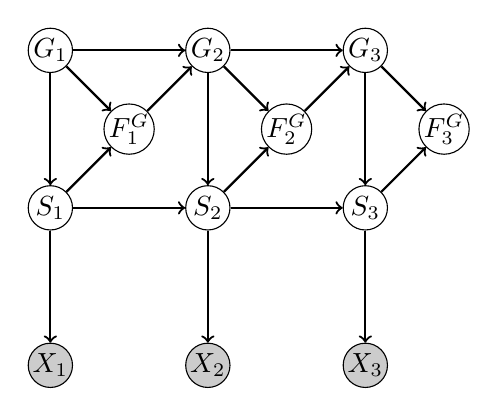
\begin{tikzpicture}[auto,swap, scale=2]
    % First we draw the vertices
    \foreach \pos/\name in {{(0, 2)/G_1}, {(1, 2)/G_2}, {(2,2)/G_3},
      {(0.5,1.5)/F_1^G}, {(1.5,1.5)/F_2^G}, {(2.5, 1.5)/F_3^G},
      {(0, 1)/S_1}, {(1, 1)/S_2}, {(2, 1)/S_3}} 
      \node[vertex] (\name) at \pos {$\name$};
    \foreach \pos/\name in {{(0, 0)/X_1}, {(1, 0)/X_2}, {(2, 0)/X_3}}
      \node[observed-vertex] (\name) at \pos {$\name$};
    % Connect vertices with edges and draw weights
    \foreach \source/ \dest in {G_1/S_1, S_1/X_1, G_1/F_1^G, S_1/F_1^G,
                  F_1^G/G_2, G_1/G_2, G_2/S_2, S_2/X_2, G_2/F_2^G,
                  S_2/F_2^G, F_2^G/G_3, G_2/G_3, G_3/S_3, S_3/X_3,
                  G_3/F_3^G, S_3/F_3^G, S_1/S_2, S_2/S_3} 
      \path[directed-edge] (\source) -- (\dest);
  \end{tikzpicture}
  \caption{A 1-level AHMM. $F_t^G$ turns on if state $S_t$ satisfies goal
  $G_t$; this causes a new goal to be chosen. However, the new state may depend
  on the old state; hence there is no arc from $F_{t-1}^G$ to $S_t$ to
  ``reset'' the submodel \cite{murphy02}.}
  \label{fig:amms}
\end{figure}

\section{Hidden Markov Model}
We use discrete hidden states to represent sub-stages of gestures.

\subsection{Emission Probability}
We use mixture of Gaussians (MoGs) emission probability with diagonal
covariances, i.e.,
\begin{align}
e(\underline{x} | s) = \sum_{m=1}^k q(m | s)\mathcal{N}(\underline{x};
\mu_{s,m}, \Sigma_{s, m})
\end{align}

The covariance has a fixed prior of $0.01\times I$ which is added to the maximum likelihood
estimate to prevent the covariance from shrinking to a point/delta function.

\begin{figure}
\centering
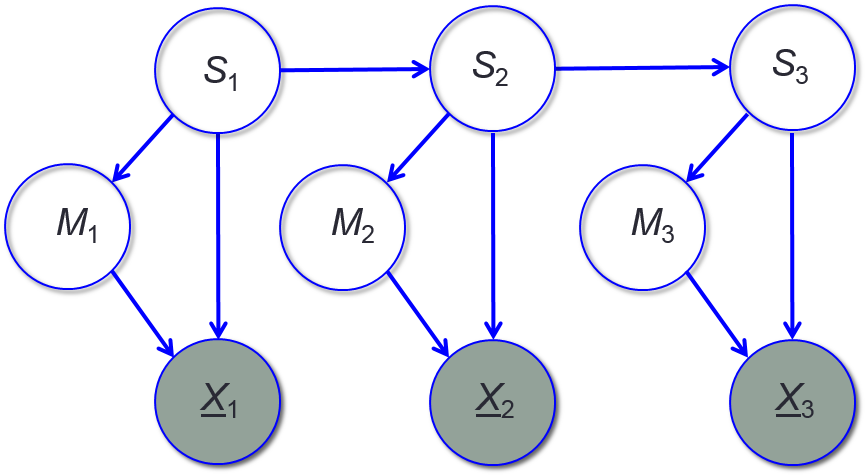
\includegraphics[width=0.5\columnwidth]{figures/mog.png}
\caption{Dynamic Bayesian network representation of HMM with mixture of
Gaussians emission probabilities.}
\end{figure}

The mixture of Gaussians parameters are initialized using K-means algorithms.
And number of number of mixtures are determined using BIC.

\subsection{Termination Probability}
As each phase can have variable length, we model the termination probability for each
hidden state $s$ as $t(\text{END}|s)$. Given a sequence of observation $\underline{X}_1^T = \underline{x}_1\ldots\underline{x}_T$, and 
the corresponding hidden states sequence $S_1^T = s_1\ldots s_T$, we define the probability
\begin{displaymath}
p(\underline{X}_1^T, S_1^T;\underline{\theta}) = 
    t(s_1)t(END|s_T)\prod_{t = 2}^T t(s_t | s_{t-1})\prod_{t = 1}^T e(\underline{x}_t|s_t)
\end{displaymath}
where $\underline{\theta}$ represents the model parameter vector which includes
the initial state probabilities $t(s)$, the state transition probabilities $t(s'|s)$, and the 
emission probabilities $e(\underline{x}|s)$ for $s, s'\in \{1, 2,\ldots k\}$. 
We use a mixture of 6 Gaussians for the emission probability to model user variations.

Given $N$ training sequences, we use the expectation maximization (EM) algorithm to estimate the model parameters. In
particular, the update for the termination probability during the $i$th iteration is 
\begin{displaymath}
t^i(END|s) = \frac{\sum_{j = 1}^N \overline{count}(j, s\rightarrow END;\underline{\theta}^{i-1})}
    {\sum_{j = 1}^N\sum_{s'} \overline{count}(j, s\rightarrow s';\underline{\theta}^{i-1})}
\end{displaymath}
where $\overline{count}(j, s\rightarrow END;\underline{\theta}^{i-1})$ is the expected count of 
$s$ being the end state. We can use the usual forward-backward algorithm to compute all the 
expected sufficient statistics by adding a dummy END state to the end of each sequence.

Because there are 3 rest positions, we use 3 hidden states for both the pre-stroke and post-stroke phases.
Each hidden state can be the start state and can only remain in its own state or go to the end state.
 
For the nucleus phase, we use 6 hidden states (chosen through cross validation) for all the gestures and use a modified Bakis~\cite{bauer2000} model to constrain the transition probabilities
among the hidden states. Instead of allowing only left-right transition, we allow the last hidden state
to go back to the initial state (Figure~\ref{fig:bakis}). This is particularly important for modeling gestures with arbitrary number of
repetitions such as waving and shaking hands. 

When initializing the transition matrix, it is important to make the possible
transitions for each state the same, so that no states are favored arbitrarily.

\subsection{Simple HMM for rest and static hand pose gestures}
One ``rest'' hidden state, transition probability = 1, termination probability =
0.5.

The self-arc on a state in an HMM defines a geometric distribution over waiting
time \cite{murphy02}. Specifically, the probability we remain in state $i$ for
exactly $d$ steps is $p(d) = (1 - p)p^{d - 1}$, where $p = A(i, i)$ is the
self-loop probability. This means the expected number of steps remaining in
state $i$ is $\frac{1}{1 - p}$.

Self-arc on a state provides smoothing, i.e., more likely to stay in the same
state.

For the rest position, let $t$ be the termination probability of a rest state.
If we assume the minimum duration of rest is 1s (30 frames), 
\begin{align}
\frac{1}{t} > 30 \\
t < \frac{1}{30}
\end{align}

\tikzstyle{vertex}=[circle, draw, minimum size=16pt, inner sep=0pt]
\tikzstyle{observed-vertex}=[circle, draw, minimum size=16pt, inner
sep=0pt, fill=black!20] 
\tikzstyle{edge} = [draw, thick, -]
\tikzstyle{directed-edge} = [draw, ->]

\begin{figure}[tb]
\centering
  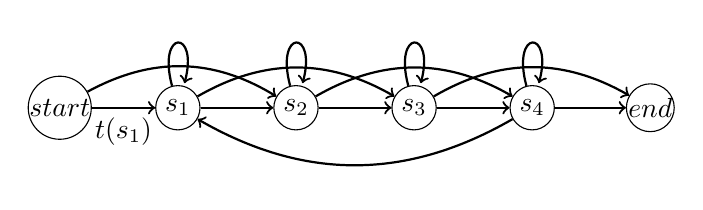
\begin{tikzpicture}[auto,swap, scale=1.5]
    % First we draw the vertices
    \foreach \pos/\name in {{(0, 0)/start}, {(1, 0)/s_1}, {(2, 0)/s_2},
    {(3, 0)/s_3}, {(4, 0)/s_4}, {(5, 0)/end}}
      \node[vertex] (\name) at \pos {$\name$};
    % Connect vertices with edges and draw weights
    \foreach \source/ \dest in {s_2/s_3, s_3/s_4, s_4/end,
    s_1/s_2} \path[directed-edge] (\source) -- (\dest);
    
    \foreach \source/ \dest in {s_1/s_3, start/s_2, s_2/s_4, s_3/end, s_4/s_1} 
      \path[directed-edge] (\source) edge [bend left] (\dest);
      
    \foreach \source/ \dest in {s_1/s_1, s_2/s_2, s_3/s_3, s_4/s_4} 
      \path[directed-edge] (\source) edge [loop above] (\dest);
    
    \path[directed-edge] (start) edge node [below] {$t(s_1)$} (s_1);
  \end{tikzpicture}
  \caption{A state transition diagram of a modified 4-state Bakis model for the nucleus phase.}
  \label{fig:bakis}
\end{figure}

\subsection{Gesture Recognition}
During the recognition phase, we concatenate the HMMs trained for each phase together to form
one HMM for each gesture. The transition probability from the previous phase to the next
phase can be computed by multiplying the termination probabilities of the previous phase and the
initial state probabilities of the next phase. Using the superscript $c$ to denote the model
parameters in the concatenated HMM, we have
\begin{displaymath}
t^c(s_\text{nucleus}|s_\text{prestroke}) = t(\text{END}|s_\text{prestroke}) \times t(s_\text{nucleus})
\end{displaymath}
where $s_{\text{phase}}$ denotes the hidden state variable in a particular phase. We add small transition
probabilities from the pre-stroke phase to the post-stroke phase to model movements that do not have the 
nucleus phase.

As new state transition probabilities are added, the transition probabilities among
states in the same phase also need to be modified so that $\sum_{s' = 1}^K t(s'|s) = 1$ (where
$K$ is the total number of combined hidden states) is ensured. For example
\begin{displaymath}
t^c(s'_{\text{nucleus}} | s_{\text{nucleus}}) = t(s'_{\text{nucleus}} | s_{\text{nucleus}})
  \times (1 - t(\text{END} | s_{\text{nucleus}}))
\end{displaymath}

We also add a rest state to the end of the HMM and allow the rest state to transit to the pre-stroke
and the post-stroke phase with uniform probabilities (Figure~\ref{fig:hmm}) to accommodate short pauses during the gesture.
As a result, the final HMM for each gesture has 13 hidden states.
Let $\underline{\theta}_g$ be the final concatenated HMM parameters for gesture $g$. The classification
of an observation sequence from non-rest positions is 
\begin{displaymath}
\hat{g} = \arg\max_g\log p(\underline{X}_1^T; \underline{\theta}_g)
\end{displaymath}


\section{Real-Time Continuous Gesture Recognition}
The temporal model of gestures can be represented by a stochastic state machine.
Each gesture phase can in turn also be represented by a stochastic state
machine, with each state generating an observation (i.e. the feature vector).
This process can be viewed as a hierarchical HMM (HHMM) (Fig.~\ref{fig:hhmm}). If we assume
that the states in the sub-HMMs are not shared, we can collapse the hierarchical HMM
into a one-level HMM for fast inference, as the graphical model for one-level
HMM does not have loops.

\begin{figure}[!t]
\centering
\includegraphics[width=0.7\columnwidth]{fig/hhmm.ps}
\caption{State transition diagram of the hierarchical HMM representation of
gesture phases. Double-ringed states are end states.}
\label{fig:hhmm}
\end{figure}

\begin{figure}[!t]
\centering
\includegraphics[width=0.7\columnwidth]{fig/embedded.ps}
\caption{Embedding phase HMMs into an entire gesture.}
\label{fig:embed}
\end{figure}

If we have ground truth labels for the pre-stroke, the nucleus and the
post-stroke phases, we can train the sub-HMMs for each phase and each gesture
separately and then combine them \cite{yin13}. However in practice, for example
if we want users to be able to easily add their new gestures by giving a few
examples, it will be tedious to manually label the start and the end of the
three phases. In this case, we can do embedded training \cite{young1994}, i.e.
train each phase sub-HMM embedded in an entire gesture segment
(Fig.~\ref{fig:embed}).

\subsection{Unified Framework}\label{sec:unified}
We do not treat the two forms of gestures separately: gestures with
distinct paths and gestures with distinct hand poses are handled within a
single probabilistic framework. This avoids making early hard decisions (which
form of gesture it is) which will be hard to correct later. Instead, we want to
make a decision only when a response is needed, according to the flow of the
current most likely gesture, and propagate beliefs as probabilities as time progresses.

\subsubsection{Gestures with distinct paths}
We use embedded training to
combine the three gesture phases together and use normal Baum-Welch algorithm to compute the
maximum likelihood of the parameters. 

Through cross-validation, we choose to use one hidden state for pre-stroke and
post-stroke phases. We use the Bakis (left-right) model \cite{Bauer00} for the
nucleus phase, but add a backward transition from the last hidden state to the first
one for gestures with an arbitrary number of repetitions (e.g., ``wave''
gesture). We use a mixture of Gaussians to model the emission probabilities for
each hidden state. We also estimate the termination
probabilities as in \cite{yin13}.

\subsubsection{Gesture with distinct hand poses}
We use one hidden state to represent this form of gestures. Let
$s_{\text{pose}}$ be the single hidden state for the nucleus phase for a gesture
with a distinct hand pose (Fig.~\ref{fig:single}). 
 Within a user,
there may be variation in the hand pose for a gesture with distinct hand pose. For example, the ``point'' hand pose can have different orientations. 
Hence, we also use a mixture of Gaussians for the emission probability
$e(\underline{x} | s_\text{pose})$.

Instead of doing embedded
training, we directly compute the maximum likelihood estimates of the mixture of
Gaussians parameters for emission probability of  $s_{\text{pose}}$. Let
$\underline{x}_1^T$ be a sequence of feature vectors corresponding to a gesture with a distinct hand pose. 
The feature vector sequence also contains random variations in the hand movement
path. 
We use Expectation Maximization (EM) to estimate the means, covariance matrices
and mixture probabilities for the mixture of Gaussians.

Since there is only one hidden state for $s_{\text{pose}}$, its transition
probability is 1. Its termination probability is estimated according to the
expected duration of the gesture. The self-arc on a state in an HMM defines a 
geometric distribution over waiting time \cite{murphy02}. In the case of a
single state HMM, the probability of remaining in state $s_{\text{pose}}$ for
exactly $d$ steps is $P(d) = p(1-p)^{d - 1}$, where $p = P(END|s_\text{pose})$
is the termination probability for $s_{\text{pose}}$. This means the expected
number of steps remaining in state $s_{\text{pose}}$ is $\frac{1}{p}$. We assume
that the minimum duration of a gesture with distinct hand pose is one second
(30 frames). The termination probability $P(END|s_\text{pose})$ is then set to
be less than $1/30$.

\begin{figure}[t]
\centering
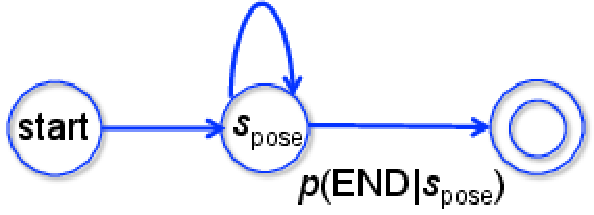
\includegraphics[width=0.5\columnwidth]{fig/single_state.ps}
\caption{State transition diagram of a single state HMM for gestures with
distinct hand poses. }
\label{fig:single}
\end{figure}

We also use one hidden state to model the rest position in a similar way.

It is possible that a gesture with a distinct path also has the same hand pose
as another gesture with distinct hand pose, for instance, some user may prefer
to do the ``circle'' gesture with a point hand pose. In this case, the gesture
will be recognized as the ``circle'' gesture because it matches both the hand
pose and the path and thus the ``circle'' gesture would have a higher likelihood
after considering a few consecutive frames.

\subsection{Real-Time Recognition}
We train the HMMs separately for each gesture, then combine them into the
hierarchical structure shown in Fig.~\ref{fig:combined}, assuming uniform
transition probabilities among gestures.
We allow sharing of the hidden states for pre-stroke and post-stroke phases for all the gestures. 

The hierarchical model allows us to do simultaneous segmentation and
recognition. We want to avoid doing segmentation first and then find the most
likely HMM for the given sequence, because segmentation based on
differentiating rest position versus non-rest position will not allow the system
to respond fast enough. We want the system to respond at the beginning of the
post-stroke phase rather then at the beginning of the rest position. In
addition, making a hard decision on segmentation can introduce errors that
are hard to correct later. 

For fast inference, we
flatten the hierarchical HMM into a regular HMM by creating an HMM state for
every leaf in the HHMM state transition diagram \cite{murphy02}. Each
hidden state $s_{GPN}$ in the flattened HMM can be indexed by three variables:
$G$ is the gesture it belongs to, $P$ is the phase it belongs to, and $N$ is its
position in the left-right model. For example, hidden state $s_{1n2}$ represents the
second hidden state in the nucleus phase of gesture 1.

\begin{figure}[t]
\centering
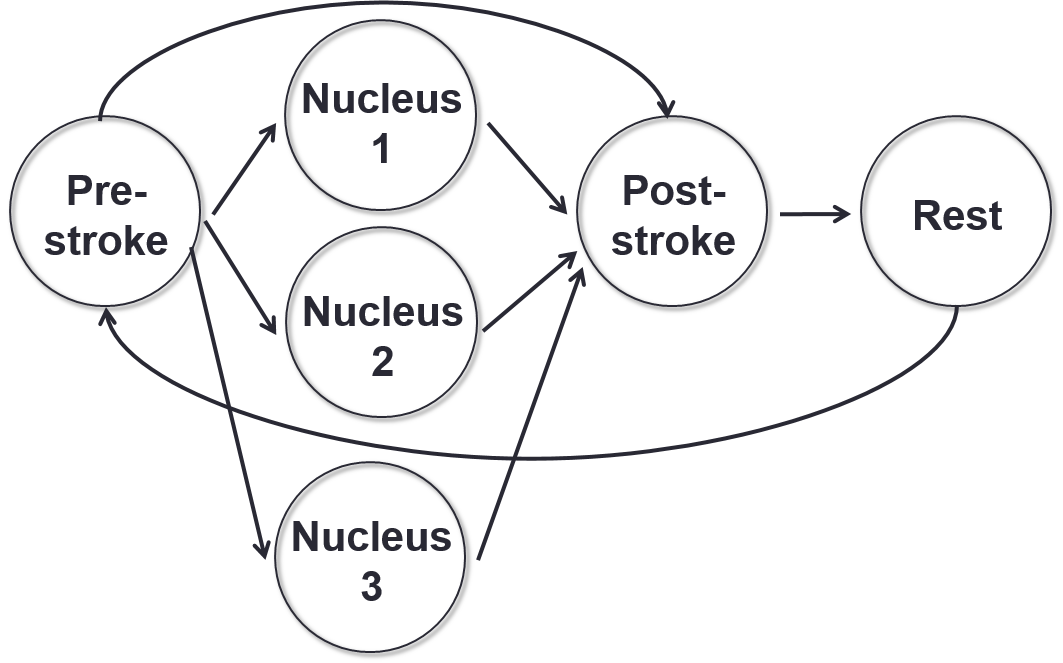
\includegraphics[width=0.7\columnwidth]{figures/combined.png}
\caption{Hierarchical HMMs for all gestures.}
\label{fig:combined}
\end{figure}

\subsection{Online Inference}
Once we have a trained model, we use fixed-lag smoothing \cite{murphy02} to do
online inference on the flattened HMM for real-time gesture recognition.
Fixed-lag smoothing is a modified forward-backward algorithm. Unlike online
filtering, which estimates the belief state at current time $t$ using forward
pass only, we estimate the state at $t - L$, given all the evidence up to the
current time $t$, i.e., compute $\gamma_{t - L}(s) \eqdef P(S_{t -
L} = s|\underline{x}_{1:t})$, where $L > 0$ is the lag. Introducing lag time is
a tradeoff between accuracy and responsiveness. Using some future evidence to
smooth the estimate can increase the accuracy while adding some delay. However
if the delay is small, it might be unnoticeable.
In the Experiment Evaluation section (Section~\ref{sec:evaluation}), we show
details about the relationship between $L$ and the recognition performance.

Fixed-lag smoothing can be implemented efficiently. We compute forward
probabilities $\alpha_t(s) \eqdef P(S_t = s|\underline{x}_{1:t})$
normally\footnote{It is more common (see e.g.,~\cite{Rabiner90}) to define
$\alpha_t(s) = P(S_t = s, \underline{x}_{1:t})$; the difference is discussed in
Section~\ref{sec:hmm-infernece}.} and keep a history window of
$\alpha_{t - L}\ldots\alpha_t$.
At every time frame, we compute backward probabilities $\beta_{t-l}(s)\eqdef
P(\underline{x}_{t-l+1:t}|S_{t-l}=s)$ from current time $t$ to $t - L$, i.e.,
form $l=0$ to $L$.
Then we can compute
\begin{align}
\gamma_{t - L} = \alpha_{t - L} \cdot \beta_{t - L}
\end{align}  
The time complexity at each time frame is $O(N_s^2L)$ where $N_s$ is the total
number of hidden states in the flattened HMM. Note that at time $t$, the belief
state at $t - L$ is committed, while the belief state from $t - L + 1$ to $t$ will still be revised later.

We can then compute the most likely hidden state at $t - L$:
\begin{align}
\hat{s} = \arg\max_s \gamma_{t - L}(s)
\end{align}
We map the most likely hidden state to the gesture label it
belongs to (including the rest position) and the gesture phase. In this way
we achieve simultaneous segmentation and recognition.

Gesture events are detected at the boundary of a phase change: start pre-stroke,
start gesture nucleus and start post-stroke. This information, together with the
gesture label for the nucleus phase, are sent to the application level.

\begin{figure}[t]
\centering
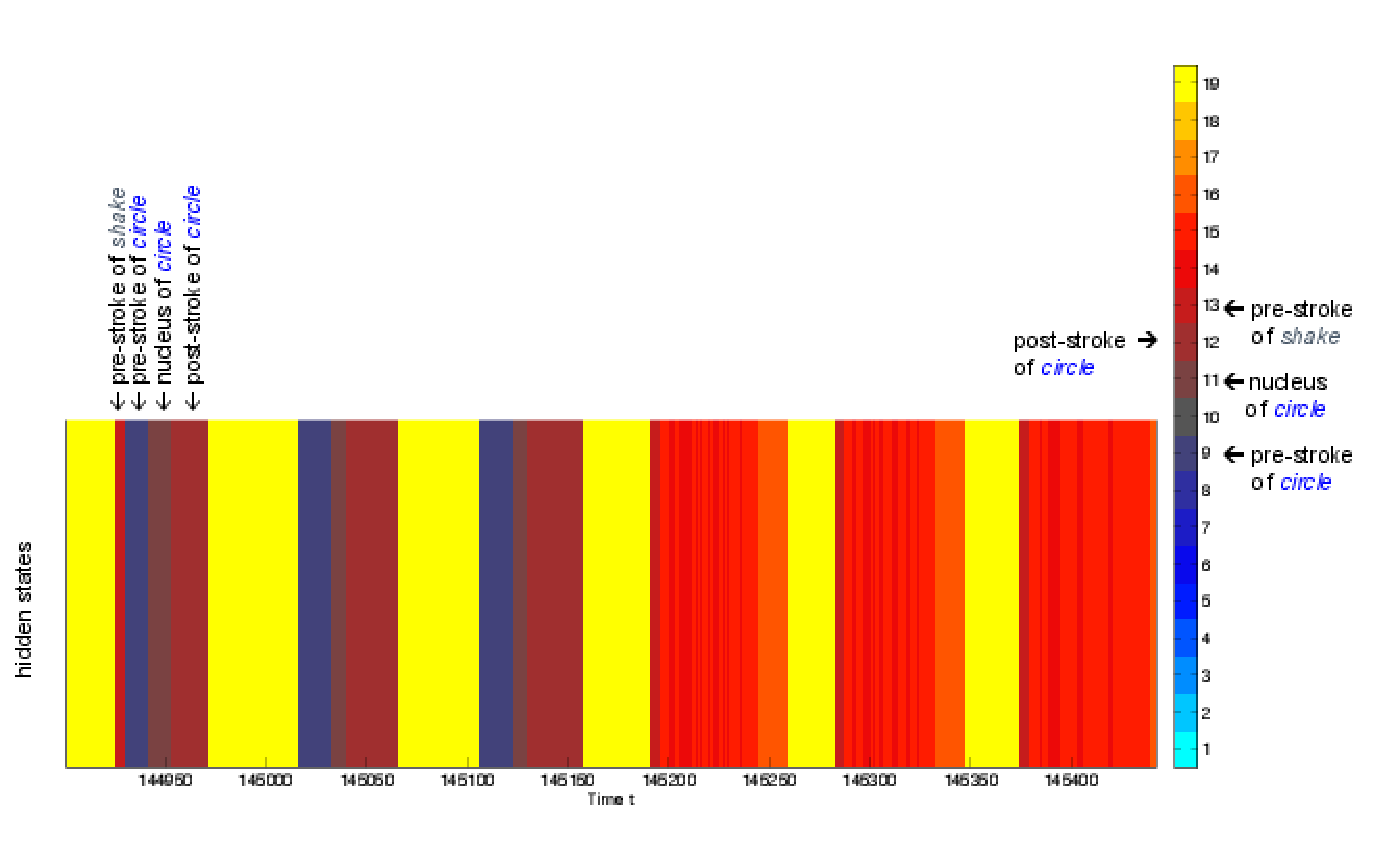
\includegraphics[trim=0 5mm 0
5mm, clip, width=1.1\columnwidth]{fig/circle_shake_label.ps}
\caption{Most likely hidden states using fixed-lag smoothing. Different colors indicate different hidden states. Yellow indicates rest position.}
\label{fig:visual_hidden}
\end{figure}

Fig.~\ref{fig:visual_hidden} shows a visualization of the
most likely hidden states based on the online fixed-lag smoothing inference
with $L = 5$.
This is based on an input sequence of 6 gestures. The first 3 gestures are
``circle'' and the last 3 gestures are ``shake hand'' gestures. Notice that in
the first segment, at the beginning, the most likely hidden state is the
pre-stroke for ``shake hand'', but since we do not need to respond at this time,
the wrong estimate does not matter. After a few more frames, the estimates are
updated to have the correct most likely gesture label and the system
responds correctly when it detects the start of the post-stroke of ``circle''
gesture.

\subsection{Gesture Spotting}
Because the non-rest positions include both pre-stroke and post-stroke phases, we need
to detect the start of the actual gesture (nucleus). We use the Viterbi algorithm
to find the most probable hidden state sequence $\hat{s}_1\ldots\hat{s}_T$ for a given observed sequence using 
the mostly likely gesture model $\underline{\theta}_{\hat{g}}$. The start and the end time for a gesture nucleus are
the first and the last time frame $t$ where $\hat{s}_t\in s_{\text{nucleus}}$ respectively. Note that
we are able to identify whether a hidden state belongs to the nucleus phase because we trained the three phases
separately.

\begin{figure}[tb]
\centering
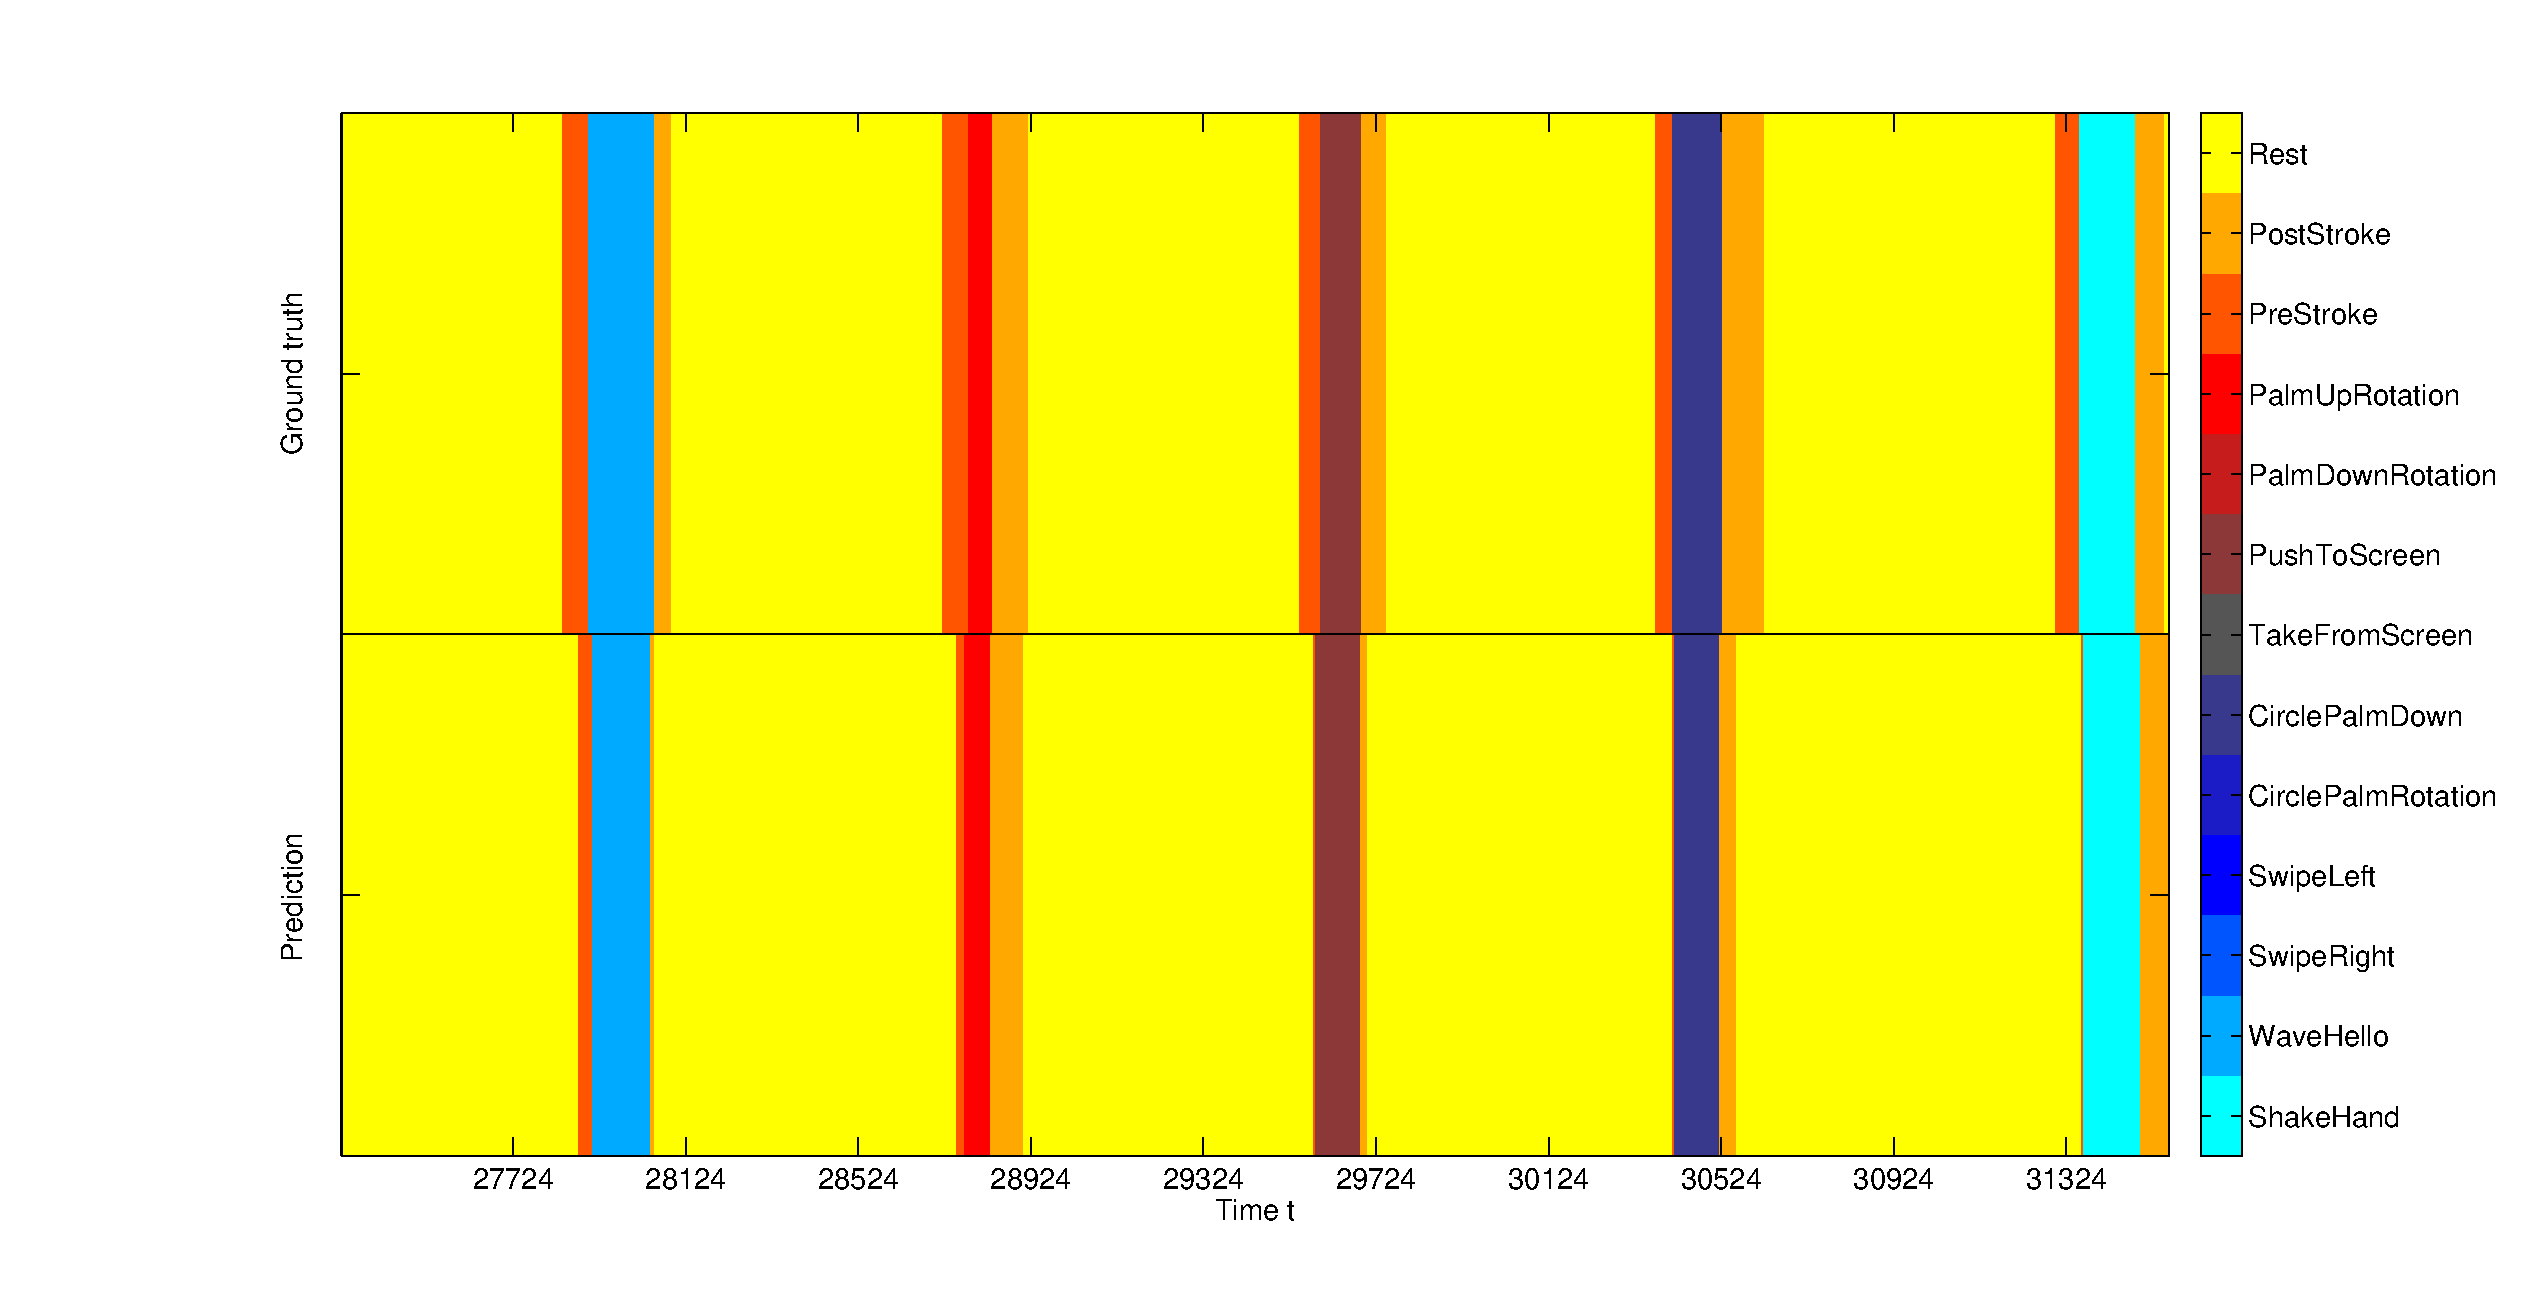
\includegraphics[trim={4cm 1cm 0cm 0.6cm}, clip,
width=1\columnwidth]{figures/gesture.eps} \caption{Visualization of a gesture
recognition sequence.
The pre-stroke and post-stroke phases are indicated by two orange colors (see the color bar).}
\label{fig:decoding}
\end{figure}

\begin{figure}[tb]
\centering
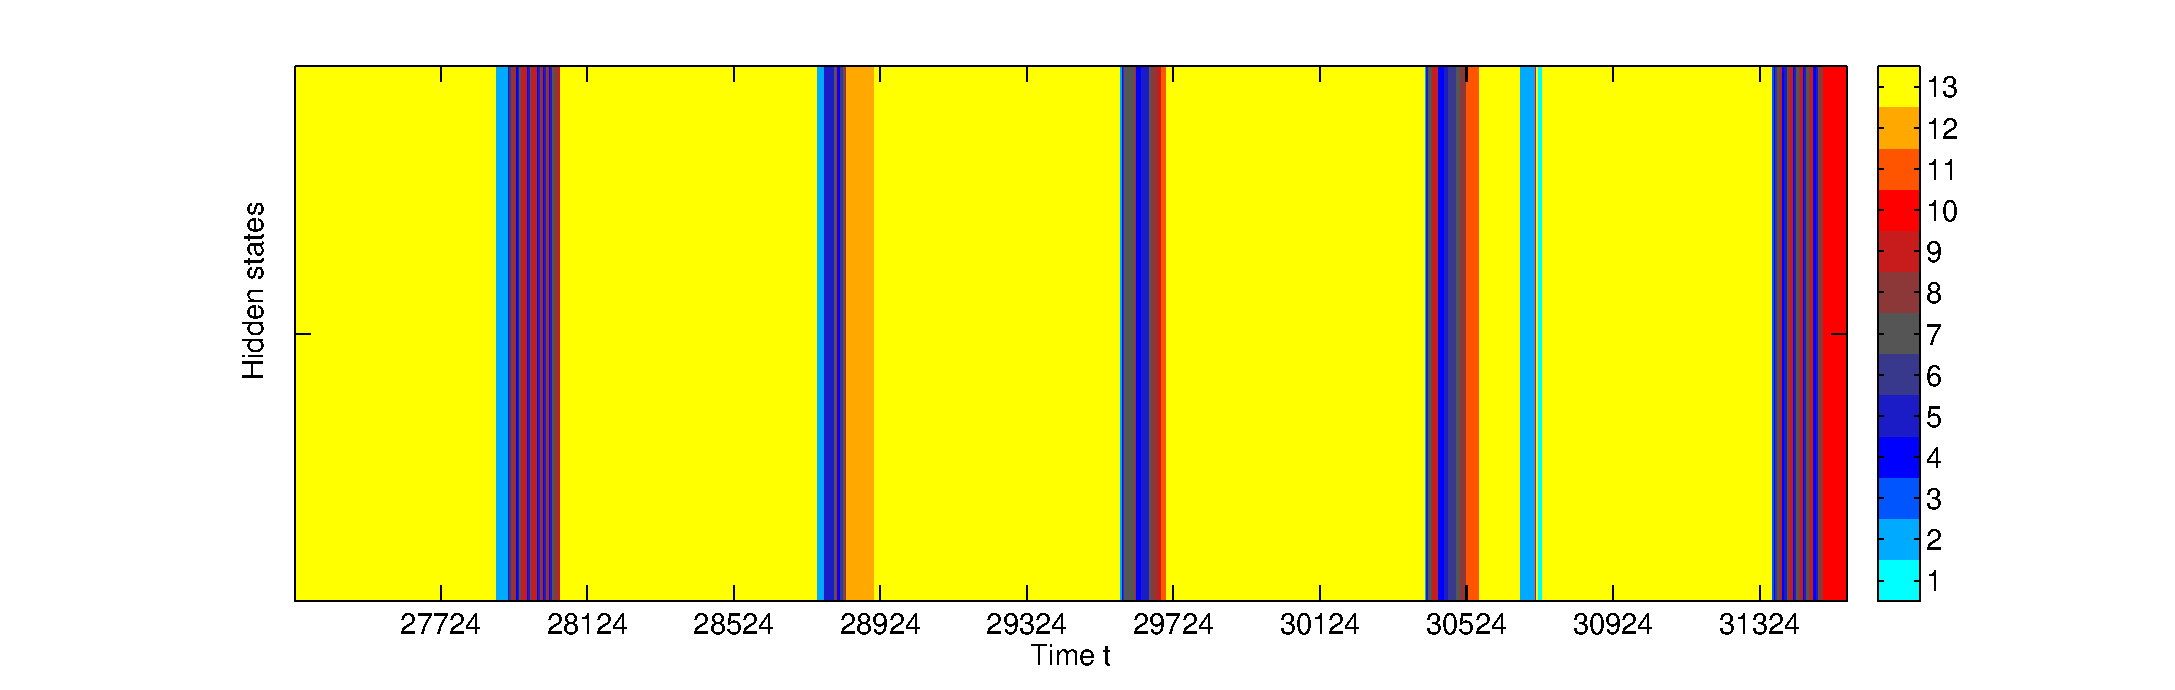
\includegraphics[trim={3.5cm 0cm 0.5cm 0cm}, clip,
width=1\columnwidth]{figures/hiddenstates.eps} \caption{Visualization of the
most probable hidden states of a gesture recognition sequence.
Colors 1-3 indicate the pre-stroke hidden states, colors 4 - 9
indicate the nucleus hidden states, colors 10 - 12 indicate the post-stroke
hidden states, and color 14 indicates the rest state.}
\label{fig:hiddenstates}
\end{figure}

Figure~\ref{fig:decoding} shows a recognition result visualization for one batch sequence. The first
row is the ground truth with different colors indicating different gesture phases or the rest position. 
The second row is our segmentation and recognition result.
Figure~\ref{fig:hiddenstates} shows the color-coded most probable hidden states
for the same sequence.
If a non-rest sequence does not contain hidden states belonging to the nucleus
phase, it is ignored (see the blue bar at $t\sim 30700$ in Figure~\ref{fig:hiddenstates}).
In this way, we can spot the actual gestures while filtering out other movements.

Compare with using likelihood information. Short sequence have higher
probability.

\section{Conditional Random Field}
LDCRF, different hidden states for different pre-stroke and post-stroke phases
for different gestures, increases computation time significantly since it
increases quadratically with number of hidden states.
Constrain transition

\section{Online Inference}
On Chairgest data.

Mention Kevin Murphy's toolbox \url{https://code.google.com/p/bnt/}